\documentclass[10pt,letterpaper]{article}
\usepackage[margin=.82in,top=.72in,bottom=.72in]{geometry}
\usepackage[T1]{fontenc}
\usepackage{lmodern,microtype}
\usepackage{amsmath,amssymb,graphicx}
\usepackage[hidelinks]{hyperref}
\setlength{\parindent}{0pt}
\setlength{\parskip}{5pt}
\hypersetup{pdftitle={Potential Across Random Permutations},pdfauthor={Jonathan R. Landers}}
\begin{document}
\begin{center}
{\Large\bfseries Potential Across Random Permutations}\\[2pt]
{\small A companion note on when disorder budgets help search}\\[5pt]
Jonathan R. Landers \qquad October 9, 2026
\end{center}

\textbf{Abstract.} The first paper bounds the cost of one search when an array's
rank-displacement potential is at most $E$; the second considers repeated searches
and a reusable index. Here we put that budget in context for a uniformly random
permutation. Exact enumeration at $n=9$ illustrates the distribution, while exact
moments and a tail bound show that a typical uniform shuffle lies beyond the point
where the potential-only displacement bound narrows the search window.

\section*{Potential under uniform shuffling}
Let $\pi=(\pi_1,\ldots,\pi_n)$ be a uniformly random permutation of the ranks
$1,\ldots,n$. The values of the underlying distinct keys do not matter. Their
disorder potential is
\[
 V_n(\pi)=\frac12\sum_{i=1}^n(\pi_i-i)^2
 =\sum_{i=1}^n i^2-\sum_{i=1}^n i\pi_i.
\]
Since $\mathbb E\pi_i=(n+1)/2$, $\operatorname{Var}(\pi_i)=(n^2-1)/12$,
and $\operatorname{Cov}(\pi_i,\pi_j)=-(n+1)/12$ for $i\ne j$,
\[
 \mu_n=\mathbb E V_n=\frac{n(n^2-1)}{12},\qquad
 \sigma_n^2=\operatorname{Var}(V_n)=\frac{n^2(n-1)(n+1)^2}{144}.
\]
Complementing every rank gives an exact pairing:
\[
 V_n(\pi)+V_n(n+1-\pi)=\frac{n(n^2-1)}6=2\mu_n.
\]
Thus the finite distribution is symmetric about its mean. It need not be
exactly normal: at $n=9$ it has two modes. A
\href{https://arxiv.org/abs/1111.3159}{combinatorial central limit theorem}
for permutation sums gives $(V_n-\mu_n)/\sigma_n\Rightarrow N(0,1)$ as $n$
grows. For a fixed tail probability $\delta$, a normal approximation suggests
$E_\delta\approx\mu_n+\sigma_n\Phi^{-1}(1-\delta)$, where $\Phi$ is the
standard normal distribution function. Exact counts are preferable in small
samples and in the tails.

\begin{figure}[ht]
\centering
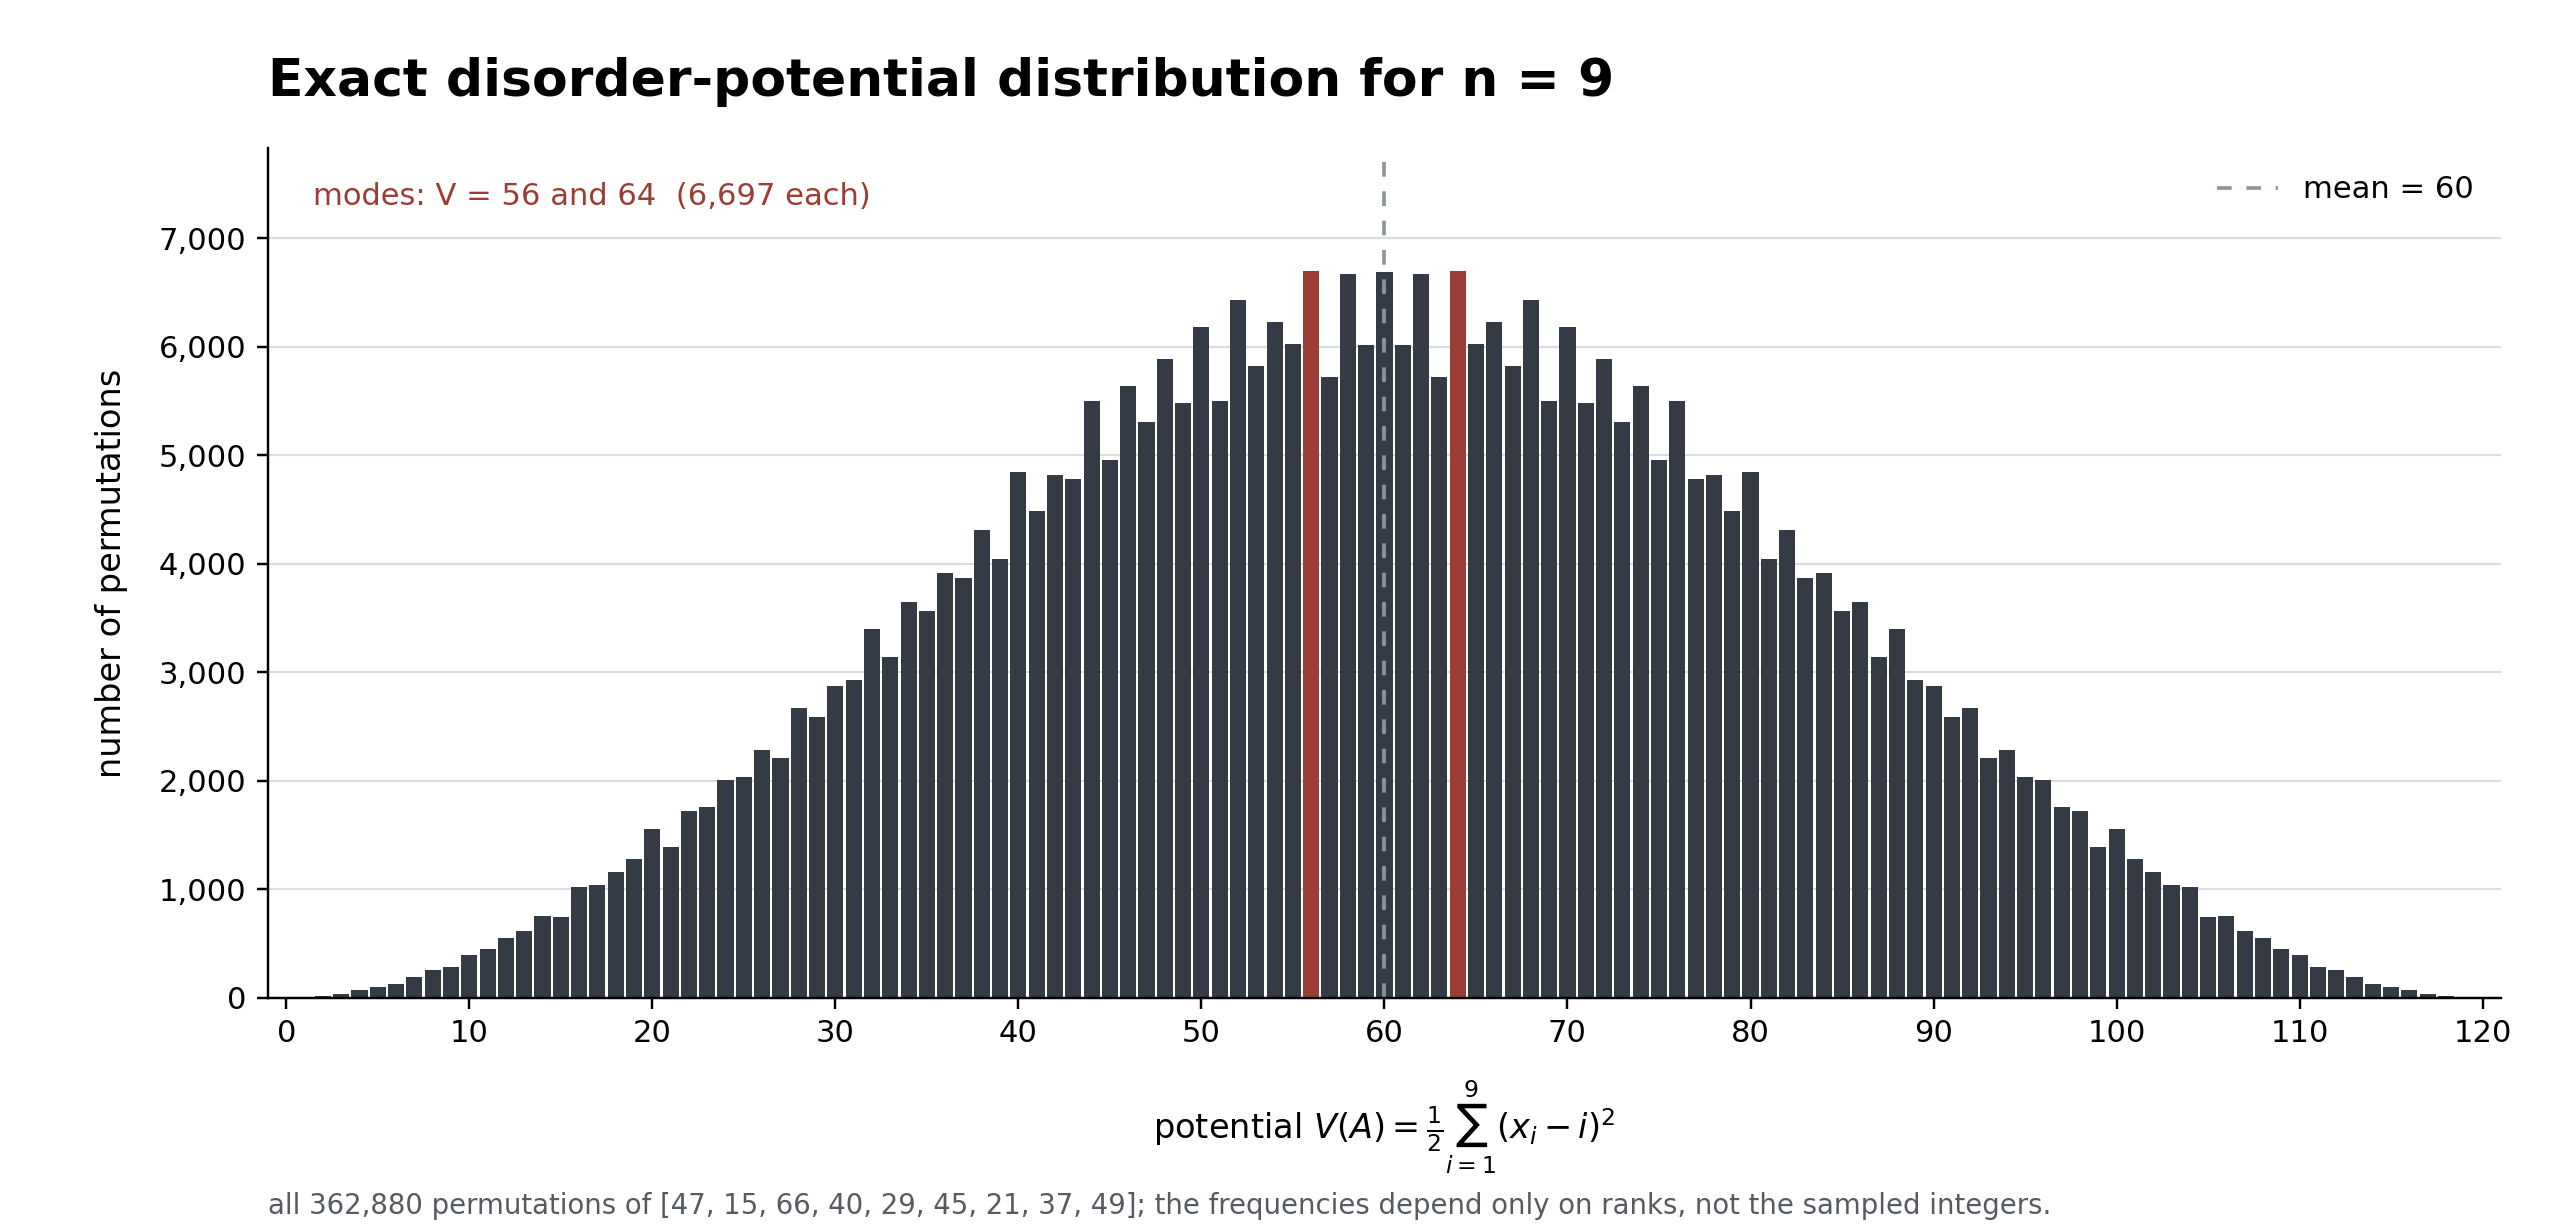
\includegraphics[width=.96\linewidth]{potential_histogram.png}
\caption{Exact counts for all $9!=362{,}880$ orderings of nine distinct keys.
Every integer potential from $0$ to $120$ occurs. The mean is $60$; the modes
are $56$ and $64$, each with $6{,}697$ orderings.}
\end{figure}

\section*{What the distribution says about search}
The \href{../../disorder_potential_search_note_v2.pdf}{first paper} proves that
a supplied promise $V(A)\le E$ gives tight worst-case one-search cost
\[
 Q^*(n,E)=\Theta\!\left(\log n+\min\{n,\sqrt E\}\right).
\]
The \href{../../search-under-a-disorder-budget/search_under_a_disorder_budget.pdf}
{repeated-search note} gives the upper bound
\[
 T_q^*(n,E)=O\!\left(q\log n+
 \min\{qR_E,\,n\log(R_E+1)\}\right),\qquad R_E=D_E+1,
\]
where the displacement certificate implied by the promise is
\[
 D_E=\min\left\{n-1,
 \left\lfloor\frac{\sqrt{1+8E}-1}{2}\right\rfloor\right\}.
\]
The distribution of $V_n$ tells us what fraction of uniform shuffles a chosen
$E$ covers. Coverage is not a certificate for an individual input: its promise
must be supplied or verified, and verification comparisons must be counted.

The displacement certificate saturates at $D_E=n-1$ when
$E\ge E_{\mathrm{sat}}=n(n-1)/2$. Yet $\mu_n\sim n^3/12$ while
$E_{\mathrm{sat}}\sim n^2/2$. For $n>5$, Chebyshev's inequality makes the
asymptotic separation explicit:
\[
 \Pr(V_n<E_{\mathrm{sat}})
 \le \frac{\sigma_n^2}{(\mu_n-E_{\mathrm{sat}})^2}
 =\frac{(n+1)^2}{(n-1)(n-5)^2}=O(1/n).
\]
At $n=9$, $E_{\mathrm{sat}}=36$ and the exact fraction below it is
$48{,}913/362{,}880\approx13.5\%$. The low-disorder cases that receive a
narrower window from this scalar certificate become rare under uniform
shuffling. Search gains for typical inputs therefore call for a distribution
favoring near-sorted arrays or a more informative description of where their
disorder lies.

\smallskip
{\footnotesize\emph{Reproduction.} The
\href{README.md}{experiment README},
\href{potential_counts.csv}{exact counts}, and
\href{plot_potential_n9.py}{enumeration script} accompany this note.}
\end{document}
